\documentclass[11pt]{article}

\usepackage[margin=0.9in]{geometry}
\usepackage[T1]{fontenc}
\usepackage{lmodern}
\usepackage{microtype}
\usepackage{amsmath,amssymb,booktabs,multirow,longtable}
\usepackage{graphicx}
\usepackage[dvipsnames]{xcolor}
\usepackage{tikz}
\usetikzlibrary{arrows.meta,positioning}
\usepackage[hidelinks]{hyperref}
\usepackage{enumitem}
\usepackage{caption}
\usepackage{subcaption}
\usepackage{cleveref}

\graphicspath{{../../outputs/}}
\setlist{nosep}
\newcommand{\AP}{\mathrm{AP}}
\newcommand{\IoU}{\mathrm{IoU}}
\newcommand{\BEV}{\mathrm{BEV}}
\newcommand{\CAV}{\mathrm{CAV}}
\newcommand{\PQSTF}{\textsc{PQ-STF}}
\newcommand{\IESTF}{\textsc{IE-STF}}

\title{Comprehensive Experimental Study of Bandwidth-Efficient\\
Cooperative LiDAR Perception}
\author{Project Progress Record}
\date{September 2026}

\begin{document}
\maketitle

\begin{abstract}
This report records the cooperative 3D perception study developed on OPV2V,
excluding an early discarded single-BEV-cell embedding baseline. The final
study combines an OpenCOOD PointPillars detector, BELT-style
uncertainty-aware box fusion, a spatial TrackFormer adaptation for cross-agent
association, geometry-noise robustness experiments, and codebook compression
of association messages. Propagated-query Spatial TrackFormer (\PQSTF)
achieves $0.891$ top-1 association accuracy on the official clean test set.
Under the canonical noisy test condition, BELT-style fusion improves
$\AP@0.7$ from $0.294$ to $0.415$, and \PQSTF association raises it to
$0.423$. Residual coding reduces the raw 1024-byte propagated query state to
roughly 2.04 bytes per selected source object with no material observed clean
test AP loss. The document separates confirmed results from incomplete
experiments and does not interpret small AP changes after compression as a
representation-quality gain.
\end{abstract}

\tableofcontents
\newpage

\section{Scope and Research Questions}

Cooperative perception allows connected autonomous vehicles (CAVs) to extend
an ego vehicle's field of view. Late fusion is attractive because each CAV
shares object-level information rather than raw LiDAR or a dense BEV feature
map. It nevertheless requires three operations: common-frame alignment,
cross-agent identity association, and robust box fusion.

The project explores these branches:
\begin{enumerate}
  \item PointPillars naive late fusion as the detector baseline;
  \item corrected localization-noise simulation and BELT-style fusion;
  \item spatial TrackFormer association at a common timestamp;
  \item clean and noise-annealed association embeddings;
  \item propagated-query and independent-embedding communication protocols;
  \item fixed, progressive residual, and uncertainty-adaptive quantization;
  \item a PQ-STF-only ablation without BELT box fusion; and
  \item a separate SWFormer sparse-transformer detector branch.
\end{enumerate}

The primary metric is average precision (AP) at 3D IoU thresholds 0.3, 0.5,
and 0.7. The strict $\AP@0.7$ metric is the primary robustness measure.
Association top-1 accuracy asks whether a source proposal's best scoring ego
proposal has the same OPV2V physical object identity.

\section{Data, Infrastructure, and Reproducibility}

\subsection{OPV2V, OpenCOOD, and cached proposals}

OPV2V supplies synchronized multi-CAV LiDAR scenes, annotations,
source-to-ego transformations, and RGB cameras. OpenCOOD supplies the
PointPillars detector, late-fusion data loader, box decoding, transforms, and
AP evaluation. The installation was adapted for the target CUDA/PyTorch
hardware before detector experiments began.

The complete training cache contains 6374 timestamps, 16,356 CAV observations,
209,251 decoded proposals, and 192,182 proposals matched to ground truth at
rotated BEV IoU $\geq0.5$. It occupies about 429 GiB because it preserves all
detector outputs required for later experiments. The official test split has
2170 evaluated timestamps.

For each proposal the cache retains scenario/frame/CAV identity, box, score,
matched object ID, GT IoU, GT box, local-to-ego transformation, and source
paths. It additionally retains the full PointPillars feature tensor, dense
classification/regression maps, and all BEV indices covered by the proposal's
rotated footprint. A materialized ROI cache was then produced to avoid
repeated scans of the 429-GiB complete cache during TrackFormer training.

\subsection{Evaluation integrity}

Noisy source boxes must use the delayed/noisy source-to-ego transformation.
An earlier late-fusion path retained source boxes but used a clean transform
during fusion, bypassing the intended noise. This was corrected before the
reported robustness experiments. We also distinguish OpenCOOD's ordinary
per-frame score ordering from optional global detection sorting: these AP
conventions must not be mixed in a direct comparison.

\section{PointPillars Detector and Naive Late Fusion}

Each CAV starts from local LiDAR points
$\mathcal{P}_i=\{(x,y,z,r)\}$. PointPillars partitions the ground plane into
XY cells; all points in one XY cell over the vertical range form a pillar. A
pillar feature network encodes nonempty pillars, scatters descriptors to a
BEV grid, and a 2D CNN backbone produces
\begin{equation}
 F_i\in\mathbb{R}^{384\times100\times176}.
\end{equation}
The $100\times176$ dimensions are BEV spatial locations, not the number of
raw LiDAR points. The 384 channels are three concatenated 128-channel
backbone branches. Detection heads predict boxes
$b_{i,k}=(x,y,z,h,w,l,\psi)$ and confidence $s_{i,k}$.

\begin{figure}[t]
\centering
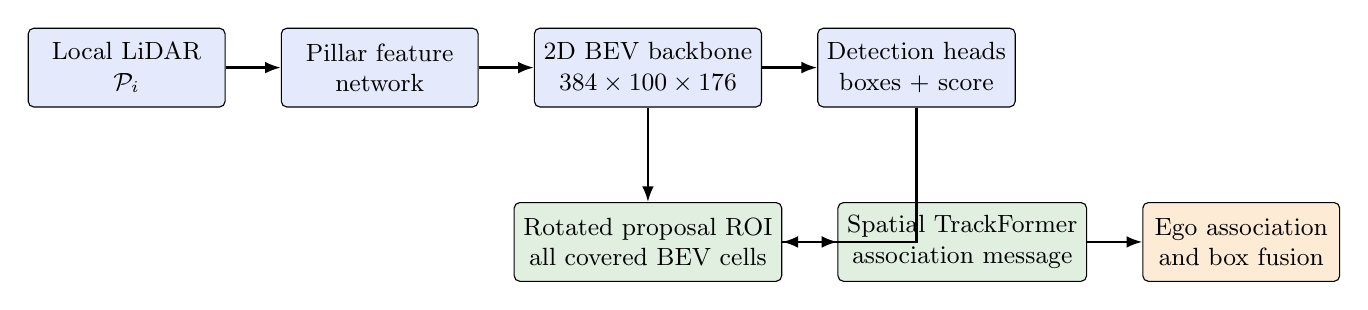
\begin{tikzpicture}[
 font=\small,
 box/.style={draw,rounded corners=2pt,align=center,minimum height=10mm,
             minimum width=25mm,fill=#1!14},
 arrow/.style={-{Latex[length=2mm]},thick},node distance=7mm]
 \node[box=RoyalBlue] (lidar) {Local LiDAR\\$\mathcal{P}_i$};
 \node[box=RoyalBlue,right=of lidar] (pfn) {Pillar feature\\network};
 \node[box=RoyalBlue,right=of pfn] (bev) {2D BEV backbone\\$384\times100\times176$};
 \node[box=RoyalBlue,right=of bev] (head) {Detection heads\\boxes + score};
 \node[box=ForestGreen,below=12mm of bev] (roi) {Rotated proposal ROI\\all covered BEV cells};
 \node[box=ForestGreen,right=of roi] (stf) {Spatial TrackFormer\\association message};
 \node[box=BurntOrange,right=of stf] (ego) {Ego association\\and box fusion};
 \draw[arrow] (lidar)--(pfn); \draw[arrow] (pfn)--(bev); \draw[arrow] (bev)--(head);
 \draw[arrow] (bev.south)--(roi.north); \draw[arrow] (head.south)|-(roi.east);
 \draw[arrow] (roi)--(stf); \draw[arrow] (stf)--(ego);
\end{tikzpicture}
\caption{Object-level cooperative perception interface. The TrackFormer
branch consumes proposal ROI cells, not the full transmitted BEV map.}
\label{fig:pipeline}
\end{figure}

Naive late fusion transforms source boxes into the ego frame, pools them with
ego boxes, and applies conventional post-processing/NMS. It transmits box
geometry and confidence only; it has no learned cross-agent identity message.

\begin{table}[h]
\centering
\caption{Clean official OPV2V test: PointPillars baseline.}
\label{tab:pointpillars}
\begin{tabular}{lccc}
\toprule
Method & $\AP@0.3$ & $\AP@0.5$ & $\AP@0.7$\\
\midrule
PointPillars naive late fusion & 0.867 & 0.859 & 0.782\\
\bottomrule
\end{tabular}
\end{table}

\section{Localization Noise and BELT-Style Fusion}

Let $T_{e\leftarrow i}$ transform a source CAV box to the ego frame. Under
localization error, alignment uses
\begin{equation}
 \tilde b_{i,k}^{(e)}=T_{e\leftarrow i}^{\mathrm{noisy,delayed}}b_{i,k}.
\end{equation}
Position noise shifts $(x,y)$ in metres; heading noise rotates $\psi$ in
degrees. Both impair strict 3D overlap, but through distinct mechanisms.

The BELT-style adapter adds evidential classification uncertainty and
heteroscedastic box covariance to frozen PointPillars. With predicted box
covariances $\Sigma_i$, associated estimates are precision weighted:
\begin{equation}
 \Sigma_f^{-1}=\sum_i\Sigma_i^{-1},\qquad
 \mu_f=\Sigma_f\sum_i\Sigma_i^{-1}\mu_i.
\end{equation}
An uncertain observation therefore has less impact on the fused box.

\begin{table}[h]
\centering
\caption{Official noisy OPV2V test: 0.2-m position noise, 0.2-degree heading
noise, 100-ms delay, seed 20.}
\label{tab:noisy-belt}
\begin{tabular}{lccc}
\toprule
Method & $\AP@0.3$ & $\AP@0.5$ & $\AP@0.7$\\
\midrule
Naive late fusion & 0.860 & 0.712 & 0.294\\
Geometry BELT fusion & 0.851 & \textbf{0.752} & 0.415\\
Geometry BELT + \PQSTF & 0.846 & 0.743 & \textbf{0.423}\\
\bottomrule
\end{tabular}
\end{table}

BELT supplies the dominant noisy recovery: $0.294\rightarrow0.415$ at
$\AP@0.7$. TrackFormer association adds a smaller strict-AP increment because
the final result also depends on box fusion and association recall.

\begin{figure}[h]
\centering
\includegraphics[width=0.82\linewidth]{belt_uncertainty_clean_test_distribution/source_proposal_uncertainty_pdf.png}
\caption{Saved uncertainty distributions. Unmatched source proposals tend to
have greater classification and localization uncertainty.}
\label{fig:uncertainty}
\end{figure}

\section{Spatial TrackFormer for Cross-Agent Association}
\label{sec:trackformer}

\subsection{Spatial adaptation of a temporal tracker}

Original TrackFormer propagates object queries from video frame $t-1$ into
frame $t$: an encoder forms memory, a decoder updates object queries, and
Hungarian matching supervises set prediction. Here, temporal context is
replaced by same-timestamp spatial context: a source CAV is analogous to the
earlier frame and ego is analogous to the current frame. This retains the
encoder--decoder and query-propagation mechanism without claiming that the
original TrackFormer performed V2X association.

For box $b_{i,k}$, let $\mathcal{R}_{i,k}$ denote its rotated proposal ROI and
let $C=|\mathcal{R}_{i,k}|$. Each ROI cell has a 384-D PointPillars vector and
a 2-D relative BEV position. The model constructs one 256-D token per cell:
\begin{equation}
 x_{i,k,r}=W_FF_i(r)+\phi_p(p_r)+\phi_g(g_{i,k}),\qquad
 X_{i,k}\in\mathbb{R}^{C\times256},
\end{equation}
where $W_F$ is a linear $384\rightarrow256$ projection, $p_r\in\mathbb{R}^2$
is a relative cell position, and $g_{i,k}\in\mathbb{R}^{9}$ contains ego-frame
box geometry and confidence. The 2-D and 9-D inputs are projected to 256-D by
learned MLPs and added to the feature projection.

The encoder self-attends over the $C\times256$ matrix, so each output cell
token contains context from all valid cells in the vehicle ROI. A learned
decoder object query attends to this memory and returns a 256-D object state
$h_{i,k}$. The association head uses that state and explicit geometry to form
a normalized 128-D embedding:
\begin{equation}
 z_{i,k}=\frac{f_\theta([h_{i,k};g_{i,k}])}
 {|f_\theta([h_{i,k};g_{i,k}])|_2}\in\mathbb{R}^{128}.
\end{equation}

\subsection{Training losses}

Original TrackFormer uses Hungarian matching between ground-truth boxes $b_i$
and predictions $\hat b_j$,
\begin{equation}
 \sigma^*=\arg\min_\sigma\sum_i\left[-\lambda_{\mathrm{cls}}
 \hat p_{\sigma(i)}(c_i)+C_{\mathrm{box}}(b_i,\hat b_{\sigma(i)})\right],
\end{equation}
where
\begin{equation}
 C_{\mathrm{box}}=\lambda_1\lVert b_i-\hat b_{\sigma(i)}\rVert_1+
 \lambda_{\mathrm{giou}}C_{\mathrm{giou}}.
\end{equation}
Matched queries receive classification and box supervision; unmatched queries
receive the no-object class. The spatial model retains the query/object logic
and adds a same-identity embedding objective. Hard negatives are nearby
vehicles with similar dimensions. The association head was trained separately
before joint use so large detection/regression losses did not overwhelm the
identity signal.

\subsection{Communication protocols}

\paragraph{\PQSTF: propagated-query Spatial TrackFormer.}
Each selected source object transmits its 256-D query state $h_{S,k}$ plus its
ordinary box geometry and confidence. Ego encodes its own ROI proposals,
injects received states as decoder queries, creates source-conditioned ego
embeddings, computes cosine similarity, and applies one-to-one Hungarian
assignment before box fusion.

\paragraph{\IESTF: independent-embedding Spatial TrackFormer.}
Each CAV independently sends a direct 128-D embedding. Ego compares source
and ego embeddings directly without a source-conditioned decoder pass. This
is cheaper to deploy but is currently less accurate end-to-end.

\begin{table}[h]
\centering
\caption{Official clean-test association evaluation.}
\label{tab:association}
\begin{tabular}{lccc}
\toprule
Protocol & Representation & Top-1 association & End-to-end $\AP@0.7$\\
\midrule
\PQSTF & propagated 256-D query state & 0.891 & 0.765\\
\IESTF (scratch) & independent 128-D embedding & 0.881 & 0.744\\
\bottomrule
\end{tabular}
\end{table}

The association-head checkpoint reached $0.915$ top-1 on held-out validation
scenarios and $0.891$ on the official clean test. It retained $0.907$ on noisy
validation and $0.891$ on the noisy test cache. Identity association remains
strong even though noisy TrackFormer GIoU and false-track metrics decline.

\begin{figure}[h]
\centering
\includegraphics[width=0.83\linewidth]{association_noise_sweep/association_top1_vs_noise.png}
\caption{Saved cross-agent association sensitivity experiment under combined
position and heading perturbations.}
\label{fig:association-noise}
\end{figure}

\section{Noise Sensitivity and Annealed Training}

Two \PQSTF association models were studied: a clean-only model and an
annealed/curriculum model trained through progressively stronger geometry-only
noise stages. Annealing trades some zero-noise specialization for slower
degradation at stronger noise; it is not expected to dominate at every point.

\begin{figure}[h]
\centering
\includegraphics[width=0.86\linewidth]{geometry_only_noise_sweep/extreme_geometry_clean_vs_curriculum.png}
\caption{Saved clean-only versus annealed association robustness experiment
under extreme combined geometry-only noise.}
\label{fig:annealing}
\end{figure}

At very high localization error, end-to-end AP curves need careful
interpretation. A source box can fail the physical association gate and remain
a singleton. The output then resembles local/non-fused detections rather than
a fully cooperative fused result. AP can therefore be non-monotonic even while
localization error increases.

\section{End-to-End Clean Results}

\begin{table}[h]
\centering
\caption{Clean official OPV2V test with fixed 5-m physical and 0.90 cosine
gates for TrackFormer variants.}
\label{tab:clean-e2e}
\begin{tabular}{lccc}
\toprule
Method & $\AP@0.3$ & $\AP@0.5$ & $\AP@0.7$\\
\midrule
Naive PointPillars late fusion & 0.867 & 0.859 & \textbf{0.782}\\
Geometry BELT fusion & 0.857 & 0.838 & 0.757\\
BELT + raw \PQSTF & \textbf{0.858} & \textbf{0.845} & 0.765\\
BELT + \IESTF (scratch) & 0.847 & 0.826 & 0.744\\
\bottomrule
\end{tabular}
\end{table}

On clean data, naive late fusion remains strongest at strict AP because boxes
are already aligned and unnecessary averaging can move a precise local box.
\PQSTF improves geometry-only BELT at strict AP ($0.757\rightarrow0.765$),
whereas \IESTF has not yet closed this gap.

\section{PQ-STF-Only Fusion Ablation}

To separate learned association from BELT box fusion, a non-BELT branch was
implemented. It uses the same \PQSTF propagated-query cosine/Hungarian
association but replaces covariance precision fusion and evidential mass
fusion by a plain detector-score-weighted box average.

\begin{table}[h]
\centering
\caption{Clean \PQSTF-only association with score-weighted box averaging.}
\label{tab:simple-pqstf}
\begin{tabular}{lccc}
\toprule
Query-state message & Bytes/object & $\AP@0.7$ & Multi-agent groups/frame\\
\midrule
Raw float32 state & 1024 & 0.7364 & 7.08\\
Fixed residual state & 4 & 0.7361 & 6.36\\
Fixed residual state & 2 & 0.7394 & 5.70\\
Fixed residual state & 1 & 0.7457 & 4.30\\
\bottomrule
\end{tabular}
\end{table}

Greater compression changes which pairs are accepted by the fixed association
rule: fewer multi-agent groups are averaged and more singleton boxes survive.
The small apparent AP increase at 1 byte is not evidence that a compressed
state is more informative. It reflects changed discrete association and fusion
decisions. Every simple-fusion result remains below naive late fusion
($0.781$ AP@0.7), confirming that BELT box fusion improves absolute quality.

The first noisy simple-fusion compression point ($1$ m position standard
deviation and $5^\circ$ heading standard deviation) is complete. Raw, 4-B,
2-B, and 1-B states obtain $0.5606$, $0.5610$, $0.5609$, and $0.5618$ AP@0.7.
Only $0.17$--$0.24$ multi-agent groups/frame remain. The remaining points
($2$ m/$10^\circ$, $4$ m/$20^\circ$, and $10$ m/$30^\circ$) are pending; no
full noisy PQ-STF-only compression curve is claimed.

\section{Codebook Quantization and Communication Cost}

Quantization applies to the \PQSTF transmitted association state $h_{S,k}\in\mathbb{R}^{256}$, not to raw LiDAR, the full BEV feature map, or the complete vehicle packet. A raw float32 query state costs
\begin{equation}
 256\times32=8192\ \mathrm{bits}=1024\ \mathrm{bytes}.
\end{equation}
Box geometry, confidence, uncertainty/rate tags, headers, and network overhead are separate fields and are excluded from these association-state payload figures.

Product quantization divides a state into subvectors and sends codebook indices. Residual product quantization sends a coarse code first and optional residual codes afterwards. Ego holds the same codebook, reconstructs $\hat h_{S,k}$, and uses it where the raw state would be used.

\begin{table}[h]
\centering
\caption{Clean test, BELT + \PQSTF, fixed residual query-state coding.}
\label{tab:fixed-quantization}
\begin{tabular}{lrrrr}
\toprule
State payload & Compression & Bytes/frame & $\AP@0.7$ & Groups/frame\\
\midrule
Raw 256-D float state (1024 B) & $1\times$ & 21935.8 & 0.76546 & 7.08\\
16-B residual state & $64\times$ & 342.7 & 0.76551 & 6.79\\
8-B residual state & $128\times$ & 171.4 & 0.76540 & 6.35\\
4-B residual state & $256\times$ & 85.7 & 0.76475 & 5.16\\
\bottomrule
\end{tabular}
\end{table}

The justified result is that propagated query states are highly compressible with no material observed clean-test AP loss over this range. Tiny non-monotonic AP changes should not be described as a representation gain.

\begin{figure}[h]
\centering
\includegraphics[width=0.84\linewidth]{pq_stf_compression_tradeoff/clean_ap70_vs_compression.png}
\caption{Saved clean-test AP@0.7 versus association-message payload. Payload means query-state bytes per selected source object.}
\label{fig:compression}
\end{figure}

\subsection{Uncertainty-adaptive residual rate}

The source CAV can select a residual prefix locally. It ranks each proposal by
classification uncertainty, predicted position standard deviation, and heading
standard deviation relative to other source proposals in that frame. Two
thresholds then choose one, two, or three residual stages. No ego feedback is
needed: source transmits a rate tag and code indices, and ego decodes the
corresponding prefix.

Validation calibration for a 1/2/4-byte codebook selected rank thresholds
$0.61$ and $0.64$. It allocated 1 byte to 62.6\% of messages, 2 bytes to
3.8\%, and 4 bytes to 33.5\%, for a mean of 2.04 bytes/object. On the official
clean test, this policy used 16.34 bits/object and 43.75 state-bytes/frame,
compared with 8192 bits/object and 21935.8 bytes/frame for raw states:
\begin{equation}
 1-\frac{16.34}{8192}=99.80\%\ \text{association-state reduction}.
\end{equation}
It obtained $\AP@0.7=0.76708$, compared with $0.76546$ raw. This $0.16$
percentage-point difference is reported as no material loss, not as an
accuracy improvement, because quantization changes discrete associations.

\begin{figure}[h]
\centering
\includegraphics[width=0.82\linewidth]{belt_uncertainty_rate_calibration_1_2_4b_validation/adaptive_rate_calibration.png}
\caption{Validation-only source-local uncertainty-rate calibration for the
1/2/4-byte residual code.}
\label{fig:adaptive-rate}
\end{figure}

\section{SWFormer Backbone Branch}

An OpenCOOD-SWFormer fork was integrated as a separate detector experiment.
Unlike PointPillars' dense 2D CNN BEV backbone, SWFormer retains occupied
voxels as sparse tokens, applies attention in regular and shifted spatial
windows, combines sparse resolutions, and uses a foreground-diffusion head.
The original method supports multi-sweep temporal input; the current OPV2V
implementation uses one LiDAR sweep per CAV.

The branch required import/extension repairs, training-resume compatibility
with current PyTorch checkpoint loading, numerical-stability work, and
batch-size memory management. Training loss became smoother, but detector AP
did not exceed the existing PointPillars checkpoint.

\begin{table}[h]
\centering
\caption{Detector branch summary on the official OPV2V test split.}
\label{tab:swformer}
\begin{tabular}{lccc}
\toprule
Detector / convention & $\AP@0.3$ & $\AP@0.5$ & $\AP@0.7$\\
\midrule
PointPillars late fusion & 0.867 & 0.859 & 0.782\\
SWFormer epoch 112, globally sorted & 0.69 & 0.69 & 0.68\\
SWFormer epoch 119, globally sorted & 0.69 & 0.69 & 0.68\\
\bottomrule
\end{tabular}
\end{table}

The much lower SWFormer result without global score sorting is a calibration/
ordering issue and must not be directly compared with a globally sorted AP.
PointPillars therefore remains the backbone for current association and
communication conclusions.

\begin{figure}[h]
\centering
\begin{subfigure}[t]{0.49\linewidth}
\centering
\includegraphics[width=\linewidth]{swformer_epoch119_eval/swformer_training_validation_loss.png}
\caption{Training and validation loss.}
\end{subfigure}
\begin{subfigure}[t]{0.49\linewidth}
\centering
\includegraphics[width=\linewidth]{swformer_epoch119_eval/pointpillars_vs_swformer_pr_curves.png}
\caption{Saved precision--recall comparison.}
\end{subfigure}
\caption{SWFormer detector branch diagnostics. Smooth loss is insufficient to
guarantee competitive detector AP.}
\label{fig:swformer}
\end{figure}

\section{Additional Tooling and Consolidated Findings}

OPV2V YAML calibration/annotation files and RGB camera images were also used to build an interactive OpenCV projection viewer. It projects LiDAR-frame 3D boxes into front/side/rear camera images, supports scenario/frame/camera navigation, filters distant and tiny boxes, and applies a basic visibility/occlusion heuristic. This is preparatory tooling for future 2D vehicle labels and visual embeddings; it is not part of current LiDAR AP.

The confirmed findings are:
\begin{enumerate}
 \item Correctly applied localization noise severely damages geometry-only late fusion; BELT-style uncertainty-aware fusion recovers a large fraction of strict AP.
 \item All vehicle-covered PointPillars ROI cells supply enough signal for strong learned association: \PQSTF reaches 0.891 clean-test top-1 accuracy.
 \item \PQSTF is currently stronger than direct independently transmitted \IESTF embeddings in end-to-end clean AP.
 \item The raw propagated query state is highly compressible. Fixed residual coding down to 4 bytes preserves clean BELT+\PQSTF AP within 0.08 percentage points of the raw-state result.
 \item Uncertainty-adaptive 1/2/4-byte coding gives a 99.80\% reduction of association-state payload with no material observed clean-test AP loss. This percentage excludes geometry, confidence, headers, and network overhead.
 \item Non-BELT score-weighted box fusion is weaker than BELT. Low-rate compression changes association/fusion decisions, so tiny AP increases must not be interpreted as a better representation.
\end{enumerate}

\subsection{Known limitations and next steps}

Clean naive late fusion is still strongest at strict AP because boxes are already aligned and averaging can be harmful. The physical association gate, NMS, and final fusion rule jointly affect AP under high localization error; association top-1 and detection AP are complementary measures. The adaptive rate policy ranks detector uncertainty but is not trained end-to-end for a rate--distortion objective. The complete noisy \PQSTF-only compression sweep is not finished beyond the first 1-m/5-degree point.

The immediate controlled work is to complete that noisy sweep, compare association-only, score-weighted, and BELT fusion using identical association settings, and compare fixed-rate and adaptive coding at matched mean payload under noise. A later multimodal branch may attach 2D visual semantic embeddings to LiDAR proposals, but it should be evaluated independently first.

\begin{thebibliography}{9}
\bibitem{opv2v} Y. Xu et al., ``OPV2V: An Open Benchmark Dataset and Fusion Pipeline for Perception with Vehicle-to-Vehicle Communication,'' 2022.
\bibitem{pointpillars} A. Lang et al., ``PointPillars: Fast Encoders for Object Detection from Point Clouds,'' CVPR, 2019.
\bibitem{trackformer} P. Meinhardt et al., ``TrackFormer: Multi-Object Tracking with Transformers,'' CVPR, 2022.
\bibitem{belt} BELT-Fusion uncertainty-aware cooperative-perception method and repository, accessed 2026.
\bibitem{swformer} SWFormer sparse-window-transformer paper and OpenCOOD-SWFormer implementation, accessed 2026.
\end{thebibliography}

\end{document}
